\section{Architecture of Zeek}
Zeek, formerly known as Bro, is a powerful network analysis tool that is distinguished by its unique architecture. This architecture is primarily divided into two major components: the event engine, which processes incoming network traffic, and the script interpreter, which applies user-defined scripts to the processed data. This high-level overview aims to elucidate the roles and functionalities of these components within Zeek's architecture.

\begin{figure}[h]
    \centering
    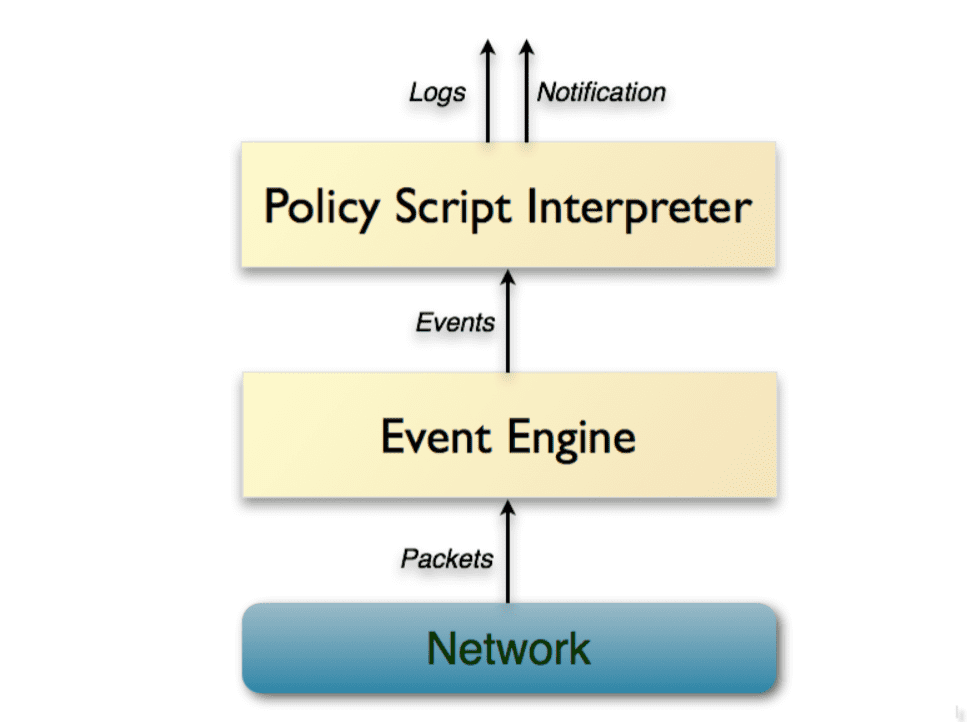
\includegraphics[width=0.5\linewidth]{images/architecture.PNG}
    \caption{Architecture of Zeek}
    \label{fig:enter-label}
\end{figure}

\subsection{Event Engine}

The event engine, or core, of Zeek plays a pivotal role in transforming the raw stream of network packets into structured, high-level events. These events are designed to be policy-neutral, focusing solely on the activities observed within the network without imparting any judgment or significance.

\subsubsection{Subcomponents of the Event Engine}

The event engine is further divided into several key subcomponents, each responsible for a specific aspect of packet processing:

\begin{itemize}
    \item \textbf{Input Sources:} This subcomponent is tasked with ingesting incoming network traffic from various network interfaces.
    \item \textbf{Packet Analysis:} Starting at the link layer, this process involves the analysis of lower-level protocols to dissect the network traffic.
    \item \textbf{Session Analysis:} Focused on application-layer protocols (e.g., HTTP, FTP), session analysis examines the content and context of communication sessions.
    \item \textbf{File Analysis:} This involves the inspection of file content being transferred over the network, providing insights into the data being exchanged.
\end{itemize}

The modularity and plugin architecture of the event engine enable the integration and expansion of Zeek's capabilities, allowing for customized enhancements beyond the core code base.

\subsection{Script Interpreter}

Complementing the event engine is the script interpreter, a critical component that leverages Zeek's custom scripting language to process the events generated by the event engine. This interpreter facilitates the implementation of a site's security policies and the derivation of network statistics.

\subsubsection{Functionality of the Script Interpreter}

The script interpreter offers a wide range of capabilities, including but not limited to:

\begin{itemize}
    \item \textbf{Security Policy Enforcement:} Through the execution of event handlers, scripts can define and enforce security measures in response to detected network activities.
    \item \textbf{Statistical Analysis:} Scripts are capable of extracting and analyzing various properties and statistics from the network traffic, enriching the understanding of network behavior.
    \item \textbf{State Management:} Zeek's scripting language allows for the maintenance of state over time, enabling the tracking and correlation of network events across different connections and hosts.
    \item \textbf{Alert Generation:} The script interpreter can produce real-time alerts and trigger external programs, facilitating proactive responses to potential security threats.
\end{itemize}



Zeek's architecture, characterized by its event engine and script interpreter, provides a robust foundation for the processing and analysis of network traffic. This design enables Zeek to deliver comprehensive insights into network activities, supporting a broad spectrum of security and monitoring applications.
